\documentclass{llncs}

\usepackage{amsmath}
\usepackage{amssymb}
\usepackage{color}
\usepackage{graphicx}
\usepackage{hyperref}
\usepackage{listings}
\usepackage{xcolor}
\usepackage{tikz}
\usetikzlibrary{arrows.meta, positioning, shapes.geometric}

\definecolor{codegreen}{rgb}{0,0.6,0}
\definecolor{codegray}{rgb}{0.5,0.5,0.5}
\definecolor{codepurple}{rgb}{0.58,0,0.82}
\definecolor{backcolour}{rgb}{0.95,0.95,0.92}

\lstdefinestyle{mystyle}{
    backgroundcolor=\color{backcolour},   
    commentstyle=\color{codegreen},
    keywordstyle=\color{magenta},
    numberstyle=\tiny\color{codegray},
    stringstyle=\color{codepurple},
    basicstyle=\ttfamily\footnotesize,
    breakatwhitespace=false,         
    breaklines=true,                 
    captionpos=b,                    
    keepspaces=true,                 
    numbers=left,                    
    numbersep=5pt,                  
    showspaces=false,                
    showstringspaces=false,
    showtabs=false,                  
    tabsize=2
}

\lstset{style=mystyle}

\newcommand{\protname}{\textsf{Matrix}}
\newcommand{\Ergo}{\textsf{Ergo}}
\newcommand{\code}[1]{\texttt{#1}}
\newcommand{\todo}[1]{{\color{red}TODO: #1}}

\newcommand{\knote}[1]{{\textcolor{green}{[kushti: #1]}}}

\begin{document}

\title{\protname{}: Splitting Ergo Blocks Into Input and Ordering Blocks For Fast Transaction Propagation and Confirmation}

\author{Alexander Chepurnoy (kushti)}
\institute{https://kushti.github.io/}

\maketitle

\begin{abstract}
This paper presents the design and implementation of \emph{Matrix}, a new design, where, instead of chain of full-blocks (which is still
being used for storing blocks beyond last few ones, bootstrapping new nodes, light clients), we have more complex structure with input and ordering blocks in Ergo.
This novel blockchain architecture separates transaction processing from block ordering to achieve faster transaction confirmations and improved
network throughput. The system introduces two types of blocks: \emph{Input Blocks} for fast transaction processing
and \emph{Ordering Blocks} for final consensus, maintaining backward compatibility through a soft-fork approach.
This architecture enables confirmation time to be in seconds range, reduces network bandwidth usage for blocks propagation, and improves scalability
without compromising security or decentralization.
\end{abstract}

\keywords{Blockchain, Scalability, Transaction Throughput, Proof-of-Work, Ergo Platform}

\section{Introduction}
\label{sec:introduction}

Trustless nature of flat peer-to-peer network~\footnote{or more efficient design reasonably close to it, such as Bitcoin network}, along
with democratic participation~(ability to run a peer software on commodity hardware with possibility to verify all the historical transactions)
is the most important property of blockchain, and must be preserved at any cost.

At the same time, fast transaction propagation and confirmations are becoming attractive properties, allowing for more
real-time like experience for payments and other financial applications. This is popularized by many financial systems
today, usually labelled as \"decentralized blockchains\", but in reality having very different topology from peer-to-peer
network powered by commodity hardware.

In this work we propose a solution, based on notable results in 15 years of blockchain research, which allows to have
faster transaction propagation and confirmation in flat commodity-hardware powered peer-to-peer networks. The proposed design
has the same security as original proof-of-work blockhain, while nearly fully utilizing network bandwidth~(and so achieving
maximum performance possible).

While the proposed solution is generic and may be applied to different Proof-of-Work networks~(probably, including
Bitcoin), in this work we focus on improving network bandwidth utilization and transaction confirmation time in Ergo network.

Talking about the Ergo network, a block is generated every two minutes on average, and confirmed transactions are propagated along with
other block sections. This is not efficient at all. Most of new block's transactions are already available in a node's mempool, and
bottlenecking network bandwidth after two minutes of (more or less) idle state is downgrading network performance (for
more, see motivation in~\cite{eyal2016bitcoinng}).

Also, while average block delay in Ergo is 2 minutes, variance is high, and often a user may wait 10 minutes for
first confirmation. Proposals to lower variance are introducing experimental and controversial changes in consensus protocol.
Changing block delay via hardfork would have a lot of harsh consequences (e.g. many contracts relying on current block
delay would be broken), and security of consensus after reducing block delay under bounded processing capacity could be
compromised~\cite{kiffer2024nakamoto}. Thus it makes sense to consider weaker notions of confirmation which still could be useful for
a variety of applications.

The rest of the paper is organized as follows. In Section~\ref{sec:architectural-overview} we outline architectural overview of the proposal. In
Section~\ref{sec:security} we provide security arguments, namely, prove that security-wise Ergo protocol will be the same after update.
In Section~\ref{sec:implementation} we provide implementation details. In Section~\ref{sec:deployment} we outline possible way for
protocol deployment. With Section~\ref{sec:conclusion} we conclude.


\section{Architectural Overview}
\label{sec:architectural-overview}

In this section, we provide overview of \protname{} design. Details are provided in the follow-up implementation section~\ref{sec:implementation}.

\subsection{Dual Blockchain Structure}
\label{subsec:dual-blockchain}

Following ideas in PRISM~\cite{bagaria2019prism}, parallel Proof-of-Work~\cite{garay2024proof}, and Tailstorm~\cite{keller2023tailstorm}, we introduce two kinds of blocks in the Ergo
via non-breaking consensus protocol update. The input/ordering blocks architecture introduces a two-tier blockchain structure as shown in Figure~\ref{fig:input-ordering-architecture}:

\begin{figure}[h]
\centering
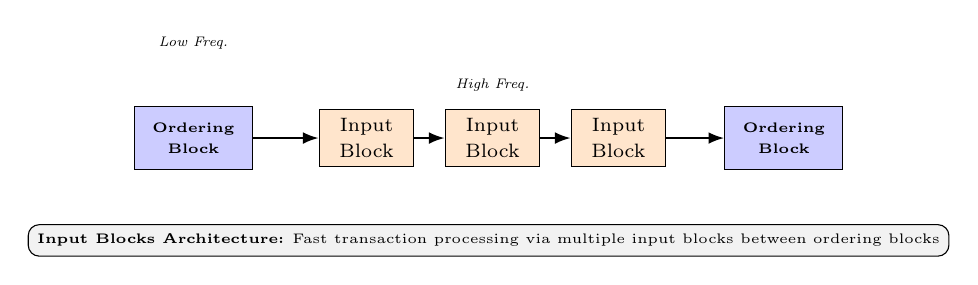
\begin{tikzpicture}[
    orderingblock/.style={rectangle, draw, fill=blue!20, minimum width=1.5cm, minimum height=0.8cm, font=\tiny\bfseries, align=center},
    inputblock/.style={rectangle, draw, fill=orange!20, minimum width=1.2cm, minimum height=0.6cm, font=\scriptsize, align=center},
    arrow/.style={-{Latex[length=2mm]}, thick}
]

% Define coordinates for the blocks (making them more spaced out)
\node[orderingblock] (ob1) at (0,0) {\shortstack{Ordering\\Block}};
\node[inputblock] (ib1) at (2.2,0) {\shortstack{Input\\Block}};
\node[inputblock] (ib2) at (3.8,0) {\shortstack{Input\\Block}};
\node[inputblock] (ib3) at (5.4,0) {\shortstack{Input\\Block}};
\node[orderingblock] (ob2) at (7.5,0) {\shortstack{Ordering\\Block}};

% Draw arrows between blocks
\draw[arrow] (ob1) -- (ib1);
\draw[arrow] (ib1) -- (ib2);
\draw[arrow] (ib2) -- (ib3);
\draw[arrow] (ib3) -- (ob2);

% Add frequency annotation
\node[above=0.1cm of ib2.north] {\tiny \textit{High Freq.}};
\node[above=0.6cm of ob1.north] {\tiny \textit{Low Freq.}};

% Add legend box at the bottom
\node[draw, fill=gray!10, rounded corners, minimum width=7cm, minimum height=0.4cm, font=\tiny] at (3.75,-1.3) {\textbf{Input Blocks Architecture:} Fast transaction processing via multiple input blocks between ordering blocks};

\end{tikzpicture}
\vspace{0.2cm}
\caption{Input-Ordering Block Architecture: Multiple input blocks (higher frequency, lower difficulty) are generated between traditional ordering blocks (lower frequency, full difficulty), enabling faster transaction confirmations.}
\label{fig:input-ordering-architecture}
\end{figure}

So instead of having just full-blocks, we have blocks of two roles here. In our design, though, this new structure is only used
for limited number of last ordering blocks, then input blocks are pruned, and ordering blocks along with input blocks they are witnessing
are compressed into full-blocks we have in the Ergo protocol right now, as illustrated in Figure~\ref{fig:compression-process}:

\begin{figure}[h]
\centering
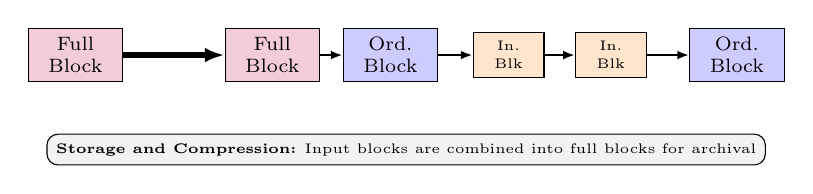
\begin{tikzpicture}[
    fullblock/.style={rectangle, draw, fill=purple!20, minimum width=1.2cm, minimum height=0.6cm, font=\scriptsize, align=center},
    orderingblock/.style={rectangle, draw, fill=blue!20, minimum width=1.2cm, minimum height=0.6cm, font=\scriptsize, align=center},
    inputblock/.style={rectangle, draw, fill=orange!20, minimum width=0.9cm, minimum height=0.5cm, font=\tiny, align=center},
    arrow/.style={-{Latex[length=1.5mm]}, thick},
    fullblockarrow/.style={-{Latex[length=2.5mm]}, line width=2pt}
]

% Define coordinates for the blocks - showing the compression process (more spaced out)
\node[fullblock] (fb1) at (0,0) {\shortstack{Full\\Block}};
\node[fullblock] (fb2) at (2.5,0) {\shortstack{Full\\Block}};
\node[orderingblock] (ob1) at (4.0,0) {\shortstack{Ord.\\Block}};
\node[inputblock] (ib1) at (5.5,0) {\shortstack{In.\\Blk}};
\node[inputblock] (ib2) at (6.8,0) {\shortstack{In.\\Blk}};
\node[orderingblock] (ob2) at (8.4,0) {\shortstack{Ord.\\Block}};

% Draw arrows between blocks
\draw[fullblockarrow] (fb1) -- (fb2);
\draw[arrow] (fb2) -- (ob1);
\draw[arrow] (ob1) -- (ib1);
\draw[arrow] (ib1) -- (ib2);
\draw[arrow] (ib2) -- (ob2);


% Legend box at the bottom
\node[draw, fill=gray!10, rounded corners, minimum width=6.5cm, minimum height=0.3cm, font=\tiny] at (4.2,-1.2) {\textbf{Storage and Compression:} Input blocks are combined into full blocks for archival};

\end{tikzpicture}
\vspace{0.2cm}
\caption{Storage Compression Process: Input blocks and ordering blocks are eventually compressed into traditional full blocks for archival storage, maintaining backward compatibility with existing Ergo infrastructure.}
\label{fig:compression-process}
\end{figure}

An input block is a by-product of mining process, i.e. they are block candidates with lower difficulty. For starters,
lets revisit blocks in current Ergo protocol, which is classic Proof-of-Work protocol formalized in~\cite{garay2024bitcoin}. A valid block
is a set of (semantically valid) header fields (and corresponding valid block sections, such as block transactions),
including special field to iterate over, called nonce, such as $H(b) < T$, where $H()$ is Autolykos Proof-of-Work
function, $b$ are block header bytes (including nonce), and $T$ is a Proof-of-Work \textit{target} value. A value which is reverse
to target is called difficulty $D$: $D = \frac{2^{256}}{T}$~\footnote{in fact, slightly less value than $2^{256}$ is being used, namely, order of
secp256k1 curve group, this is inherited from initial Autolykos 1 Proof-of-Work algorithm}. $D$ (and so $T$) is being readjusted
regularly via a deterministic procedure (called difficulty readjustment algorithm) to have blocks coming every two minutes on average.

Aside of blocks, \textit{superblocks} are also used in the Ergo protocol, for building NiPoPoWs on top of them. A superblock is
a block which is more difficult to find than an ordinary, for example, for a (level-1) superblock $S$ we may require
$H(S) < T/2$, and in general, we can call n-level superblock a block $S$ for which $H(S) < T/2^n$. Please note that a
superblock is also a valid block (every superblock is passing block PoW test).

We propose to name full blocks in Ergo as \textit{ordering blocks} from now, and use input-blocks (or sub-blocks) to carry most
of transactions. For starters, we set $t = T * 64$ (the multiplier will be revisited later) and define input-block $i$ generation
condition as $ T < H(i) < t$, then a miner can generate on average 63 input blocks plus an ordering block
per ordering block generation period. Please note that, unlike superblocks, input blocks are not passing ordering-block PoW check,
but an ordering block is passing input block check.

\subsection{Linking Structure}
\label{subsec:linking-structure}

Every input block is referencing previous input block and also parent ordering block. An ordering block is referencing
previous ordering block as well as last seen input block. In both cases, a reference to an ordering block is written into
a block header. In case of Ergo, reference to last seen input block is written into an extension section of a block, see
implementation section for details~(in an implementation for Bitcoin or a fork of Bitcoin, a coinbase transaction can be used).

Linear relationship with linking is coming along linear relationship in regards with transactions (ie no conflicts
possible between input block transactions). See the next subsection for details.

\subsection{Transactions Validation and Confirmation}
\label{subsec:transactions-validation}

Ideally, all the transactions should be in input blocks only. In a simplest blockchain with payment transactions only that would
be doable by introducing a requirement to have transactions in input blocks only. However, with rich blockchain context that would be
impossible in Ergo, as a transaction in input block may use blockchain header fields which could be different in ordering block~(timestamp, miner pubkey, votes). Then old clients which are validating ordering blocks only would fail. Thus we break transactions into two classes. Normally, we expect that about 99\% of transactions would be of class one, and they would be included into input blocks only.


\subsection{Transaction Classification}
\label{subsec:transaction-classification}

Transactions are classified into two categories based on their validation requirements:


\subsubsection{First-class Transactions}
\label{subsubsec:first-class}
\begin{itemize}
\item Validation outcome independent of block context
\item Can only be included in input blocks
\item Examples: Simple transfers, most smart contracts (which do not depend on block timestamp, miner pubkey)
\end{itemize}

\subsubsection{Second-class Transactions}
\label{subsubsec:second-class}
\begin{itemize}
\item Validation depends on block context (block timestamp, miner pubkey, block votes)
\item Can be included in both input and ordering blocks
\item Examples: emission contracts, time-dependent contracts
\end{itemize}

In the UTXO model, a transaction is second-class if a script of any input of it reads block context data
(block timestamp, miner pubkey, block votes), otherwise, the transaction belongs to first class.

\subsubsection{Fees}
\label{subsubsec:fees}

A transaction fee is not a part of the core Ergo protocol. A reference client implementation is currently recognizing
as a transaction fee contract one which is locking fee under miner's public key, and no alternative options
automatically checked. Using miner public key makes a transactions belonging to second-class transactions, and such
transactions can be included into ordering blocks only. So to bring miners transaction fees to input blocks we need to introduce additional
fee contracts. The simplest option is to use just TRUE (anyone-can-spend) proposition. It is also the best option for
compacting blockchain space.

\subsection{Block Types and Properties}
\label{subsec:block-types}

Here we summarize difference between input and ordering blocks.

\begin{table}[h]
\centering
\begin{tabular}{lcc}
\hline
\textbf{Property} & \textbf{Input Blocks} & \textbf{Ordering Blocks} \\
\hline
PoW Target & $T/64$ & $T$ \\
Frequency & 64x more frequent & Standard \\
Finality & Provisional & Final \\
Transaction Types & First-class only & All types \\
Miner Rewards & Fees + Storage rent & Emission + Fees \\
\hline
\end{tabular}
\caption{Comparison of Input Blocks and Ordering Blocks}
\label{tab:block-comparison}
\end{table}

\section{Implementation}
\label{sec:implementation}

In this section we describe how to implement input blocks without breaking current full and light Ergo clients. Our
proposal is generic enough and can be reused for other classic Proof-of-Work blockchains (such as Bitcoin).

\subsection{Extension}
\label{subsec:extension}

There are three new fields in extension field of a block:
\begin{itemize}
  \item a digest (Merkle tree root) of new first-class transactions since last input-block. Key is 0x0300,
        value is Merkle tree root bytes (32 bytes).
  \item a digest (Merkle tree root) of first-class transactions since ordering block till last input-block. Key is 0x0301,
  value is Merkle tree root bytes (32 bytes).
  \item reference to a last seen input block. Key is 0x0302, value is input block id (32 bytes).
\end{itemize}



\subsection{Proof-of-Work Inequality}
\label{subsec:pow-inequality}

Instead of one classic Proof-of-Work inequality, two are used now:

\begin{itemize}

\item{} ordering blocks maintain the traditional PoW requirement:

\begin{lstlisting}[language=Scala]
  hash(header) < Target
\end{lstlisting}

\item{} for input blocks, we use lower  difficulty, i.e. higher target, e.g. 64x of block target to have input block
generation average delay to be $\frac{1}{64} th$ of ordering (full) block delay :

\begin{lstlisting}[language=Scala]
  hash(header) < Target * 64
\end{lstlisting}

\end{itemize}

\subsection{Network Protocol Extensions}
\label{subsec:network-protocol-extensions}

The P2P network protocol is extended with new message types to support the dual-block architecture:

\begin{itemize}
\item \code{InputBlockMessageSpec} (code: 100) - Input block announcements containing header, extension fields, and weak transaction IDs
\item \code{InputBlockTransactionIdsMessageSpec} (code: 101) - Lists transaction IDs for verification against Merkle proofs in input blocks
\item \code{InputBlockTransactionsMessageSpec} (code: 102) - Transmits actual transaction data for input blocks
\item \code{InputBlockTransactionsRequest} (code: 103) - Requests specific transactions from input blocks
\item \code{OrderingBlockAnnouncement} (code: 104) - Ordering block announcements with additional input block references
\end{itemize}

These message extensions allow nodes to efficiently propagate and validate both input and ordering blocks, enabling the faster confirmation times while maintaining network security.

\subsubsection{Input Block Announcement}
\label{subsubsec:input-block-announcement}

When a miner successfully generates an input block, the following announcement procedure is executed:

\begin{enumerate}
\item The miner creates an \code{InputBlockMessageSpec} (message code 100) containing the input block header, extension fields (including the link to the previous input block), and weak transaction IDs if available.
The extension fields contain the Merkle root of new first-class transactions since the last input block (key 0x0300), the Merkle root of all first-class transactions since the parent ordering block (key 0x0301), and a reference to the previous input block (key 0x0302).
The input block is announced to peers via the P2P network.

\item Upon receiving an input block announcement, a peer node validates the PoW solution and Merkle proof against the extension root in the header.

\item If validation passes, the peer requests the corresponding transaction IDs using \code{InputBlockTransactionIdsMessageSpec} (code 101) to verify the weak transaction IDs against the extension digest.

\item The peer then downloads the actual transactions and validates them against the input block's commitment.

\item Once validated, the input block is processed and added to the appropriate input block chain or fork.
\end{enumerate}

This announcement procedure ensures rapid propagation of input blocks across the network while maintaining security through validation of PoW and transaction commitments. The separation of header announcement from transaction data allows for efficient bandwidth utilization, as most transactions are already available in the mempool.

It is possible that a peer receives an input block with a missing parent input block or ordering block. The system handles these scenarios as follows:

\begin{itemize}
\item{} when a peer receives an input block but does not have its parent input block (identified by the \texttt{prevInputBlockId} field in the extension), the peer adds the received input block to a disconnected waitlist. The peer then requests the missing parent input block from the network. Once the parent block is received and validated, the peer processes the child block from the waitlist. This can be done
recursively.

\item{} if an input block references an ordering block that is not yet known to the peer, the input block is temporarily stored in the disconnected waitlist. The peer then attempts to download the missing ordering block from the network. Once the ordering block is received and validated, the input block can be processed normally. Thus input blocks
allow to quickly find all the forks around the network and finalize a best one.

\end{itemize}

To prevent the waitlist from growing indefinitely, input blocks with missing parents are evicted after a certain timeout period if their dependencies are not resolved.

\knote{make interaction diagrams}

\subsection{Transaction Processing}
\label{sec:transaction-processing}

Transaction processing in \protname{} divides transactions into two classes based on their dependency on block context, first-class transactions
which do not use non-fixed upcoming block related context in any of input scripts, and second-class, which are doing so. Formally, a transaction is second-class if any input script accesses any of (timestamp, miner public key, block votes) fields of upcoming block; otherwise, it belongs to the first class.

Input blocks exclusively carry first-class transactions. When an input block is received, the following processing occurs:

\begin{enumerate}
\item The node validates the PoW solution and Merkle proof against the extension root in the header.
\item Transaction IDs are verified against the Merkle root of new first-class transactions since the last input block (extension field key 0x0300).
\item All transactions are validated against the current UTXO set and state.
\item Transaction costs are calculated and accumulated to ensure block limits are not exceeded.
\item Validated transactions are applied to update the UTXO set.
\end{enumerate}


Transaction dependency consistency across input block chains is maintained. In particular, that does mean following:

\begin{itemize}
\item Outputs spent in later input blocks remain available until the spending transaction is processed
\item Double-spending attempts are detected and rejected
\item Chain reorganizations properly handle transaction dependencies
\end{itemize}

\subsubsection{Fork Handling and Transaction Rollback}
\label{subsubsec:fork-handling-transactions}

When switching between competing input block forks, the system handles transaction rollback and reapplication:

\begin{enumerate}
\item When a longer competing fork is detected, transactions from the abandoned fork are marked as unconfirmed and returned to the mempool.
\item Transactions from the new best fork are applied to the state in sequence.
\item The UTXO set is updated accordingly to reflect the new transaction ordering.
\item Mempool is refreshed to remove transactions that are now confirmed in the new best chain.
\end{enumerate}

This mechanism ensures that transaction confirmations remain consistent even when input block forks are resolved.

\subsection{Chain Selection and Fork Handling}
\label{subsec:chain-selection}

Unlike DAG systems, Ergo has classic linking structure, like in Bitcoin. For ordering blocks, a chain with most
Proof-of-Work (cumulative difficulty) is considered canonical. When a new block on the same height as best one
arrives, it is not accepted as best one (so first seen is considered best). However, if better suffix of the chain
arrives, then node is rolling back its state to common block and apply the better suffix.

The same rules apply to input blocks. For ordering blocks of the same difficulty, chain with most Proof-of-Work
(cumulative difficulty) is considered best. However, for input blocks we consider not difficulty which should be met,
 but real one (which is used in NiPoPoWs), which is similar approach to PoEM (Proof of Enthropy Minima).
 For input blocks chains with the same real difficulty, one which is seen first is chosen.
 \knote{ordering block with most of input blocks difficulty is the best?}

\subsection{Light Clients}
\label{sec:light-clients}

\subsubsection{Stateless clients}
\label{subsec:stateless-clients}

Ergo has a support for partially stateless clients, where only miners need to store UTXO sets, and stateless clients
can ask stateful ones for authenticated AVL+ tree based proofs of UTXO set transformations~\cite{reyzin2017improving}.

% TODO: do we need to leave stateless clients intact or can modify

\subsubsection{SPV and NiPoPoW clients}
\label{subsec:spv-nipopow-clients}

An SPV client is not downloading full blocks, only block headers or short proof of headers-chain, such as NiPoPoW~(a
non-interactive proof of proof-of-work)~\cite{kiayias2020non}, and then ask for transactions.

Input blocks perfectly compatible with SPV clients. An SPV client can still ask for headers or NiPoPoW just, and so enjoy
the same minimal bandwidth requirements, or it may ask for input-blocks additionally, to enjoy faster confirmations.


\section{Security}
\label{sec:security}

\knote{provide formalization of security properties}


\section{Deployment}
\label{sec:deployment}

We plan to deploy \protname{} gradually:

\begin{itemize}
  \item{} First of all, only some mining pools and solo miners will implement \protname{}. They will form peer-to-peer
           sub-network which peers send input/ordering blocks related messages to other sub-network peers, but avoid
           to send them to other peers (not supporting input blocks yet). At this point extension fields do not necessarily
           present in extension section.
  \item{} More and more miners support \protname{}, and when 90+\% hashrate is on it, lock-in voting takes place.
            One-epoch indicative voting would be enough. In case of 90+\% hashrate support voting for lock-in,
            extension fields become necessary, and so \protname{} becomes part of the protocol. However, old block structure
            and p2p messages still supported, for bootstrapping nodes with historical data, and to support older as well
            as light clients.
\end{itemize}


\section{Conclusion}
\label{sec:conclusion}

The \protname{} implementation represents a significant advancement in Ergo's scalability and user experience without compromising security or decentralization. By separating transaction processing from consensus finalization, this architecture enables faster confirmations, improved throughput, and better network efficiency while maintaining full backward compatibility.

The soft-fork compatible approach ensures smooth deployment, and the innovative use of Merkle proofs and transaction classification maintains the security properties that make Ergo a robust platform for contractual money. This implementation positions Ergo at the forefront of scalable blockchain solutions while preserving its commitment to decentralization and innovative smart contract capabilities.

\section*{Acknowledgments}

The authors would like to thank the Ergo community and contributors for their support and feedback during the development of this architecture. Special thanks to the researchers whose work inspired this approach, particularly the Bitcoin-NG, Prism, and Tailstorm projects.

\bibliographystyle{plain}
\bibliography{references}

\end{document}